% algorithms: 
% views: 
% containers: adjacency matrix
% data model: incoming edges on a vertex

\chapter{Introduction}
\label{ch:introduction}


\section{Example: Six Degrees of Kevin Bacon}
\label{sec:bacon}

A classic example of the use of a graph algorithm is the game ``The Six Degrees of Kevin Bacon.''
The game is played by connecting actors to each other through movies they have appeared in together.
The goal is to find the smallest number of movies that connect a given actor to Kevin Bacon.
That number is called the ``Bacon number'' of the actor. Kevin Bacon himself has a Bacon number of 0.
Since Kevin Bacon appeared with Tom Cruise in ``A Few Good Men'', Tom Cruise has a Bacon number of 1.

The following program computes the Bacon number for a small selection of actors.
  {\small
\begin{lstlisting}
std::vector<std::string> actors { "Tom Cruise",       "Kevin Bacon",       "Hugo Weaving",
                                  "Carrie-Anne Moss", "Natalie Portman",   "Jack Nicholson",
                                  "Kelly McGillis",   "Harrison Ford",     "Sebastian Stan",
                                  "Mila Kunis",       "Michelle Pfeiffer", "Keanu Reeves",
                                  "Julia Roberts" };

std::vector<std::vector<int>> costar_adjacency_list {
    {1, 5, 6}, {7, 10, 0, 5, 12}, {4, 3, 11}, {2, 11}, {8, 9, 2, 12}, {0, 1}, {7, 0},
    {6, 1, 10}, {4, 9}, {4, 8}, {7, 1}, {2, 3}, {1, 4} };

int main() {
  std::vector<int> bacon_number(size(actors));

  for (auto&& [u, v] : bfs_edge_range(costar_adjacency_list, 1)) { // Vertex 1 -> Kevin Bacon
    bacon_number[v] = bacon_number[u] + 1;
  }

  for (int i = 0; i < size(actors); ++i) {
    std::cout << actors[i] << " has Bacon number " << bacon_number[i] << std::endl;
  }
}
\end{lstlisting}
}

In graph parlance, we are creating a graph where the vertices are actors and the edges are movies.
The number of movies that connect an actor to Kevin Bacon is the shortest path in the graph
from Kevin Bacon to that actor. In the example above, we compute shortest paths from Kevin
Bacon to all other actors and print the results.


\section{Graph Background and Terminology}

For clarity, we briefly review some of the basic terminology of graphs.
We use commonly accepted terminology for graph data structures and algorithms and
adopt the particular terminology used in the textbook by
Cormen, Leiserson, Rivest, and Stein (``CLRS'')~\cite{CLRS2022}.

\subsection{Theoretical Terminology}

A \emph{graph} $G$ is a set comprised of two other sets, the vertex set $V$ and the edge set $E$,
typically expressed as $G=\{V,E\}$. We can number the members of the vertex set
and write $V = \{ v_0, v_1, \ldots , v_{n-1} \}$. Similarly, we can write $E = \{ e_0, e_1, \ldots, e_{m-1} \}$. The number of elements in $V$ is denoted by $|V|$ and the number of elements in $E$ is denoted by $|E|$. Edges in $E$ are pairs of vertices; for any $e_k \in E$, we write $e_k = ( v_i, v_j )$, where $v_i \in V$ and $v_j\in V$. The edges in $E$ may be \emph{uordered}, in which case $(v_i, v_j) = (v_j, v_i)$ or \emph{ordered}, in which case $(v_i, v_j) \neq (v_j, v_i)$ (unless $i = j$).
A graph consisting of unordered edges is said to be \emph{undirected};
a graph consisting of ordered edges is said to be \emph{directed}.
Since there is a single set of vertices in this definition of $G$, that is, edges connect
vertices in $V$ to vertices in $V$, we say that
$G$ is a \emph{unipartite} graph.
If the graph further has no loops (edges connecting a vertex to itself)
and no multiple edges (edges connecting the same pair of vertices),
then $G$ is called a \emph{simple} graph.
A \emph{complete graph} is a simple graph $G$ where every vertex is connected
to every other vertex; a complete graph has
$n$ vertices and $n(n-1)/2$ edges.
A \emph{path} is a sequence of vertices $v_0, v_1, \ldots, v_{k-1}$ such that
there is an edge from $v_0$ to $v_1$, an edge from $v_1$ to $v_2$, and so on.
That is, a path is a set of edges $(v_i, v_{i+1}) \in E$ for all $i = 0, 1, \ldots, k-2$.

Graphs are often deipicted as a collection of nodes and links, as shown in
Figure~\ref{fig:node_link_graphs}. In this model, vertices are
represented graphically as nodes, which are
shown as circles (or some other shape, including points). Edges are represented as links,
shown as lines connecting the nodes.


\begin{figure}[ht]
  \begin{center}
    \subcaptionbox{An undirected graph representing airline routes between cities.\label{subfig:airport}}
    {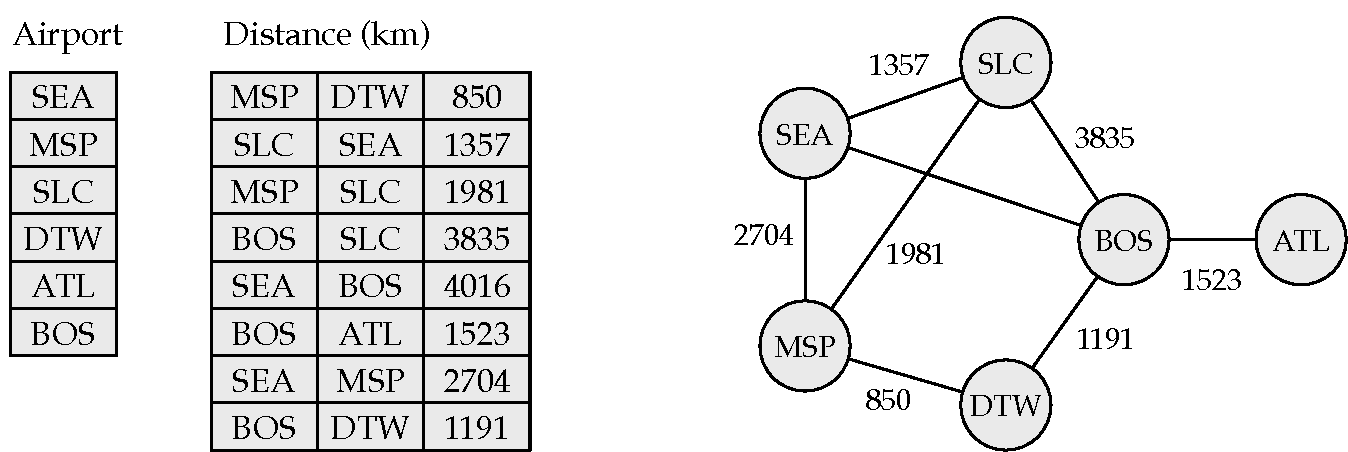
\includegraphics[width=0.42\textwidth]{figs/airport.pdf}}
    \subcaptionbox{A directed graph representing an electronic circuit.\label{subfig:circuit}}
    {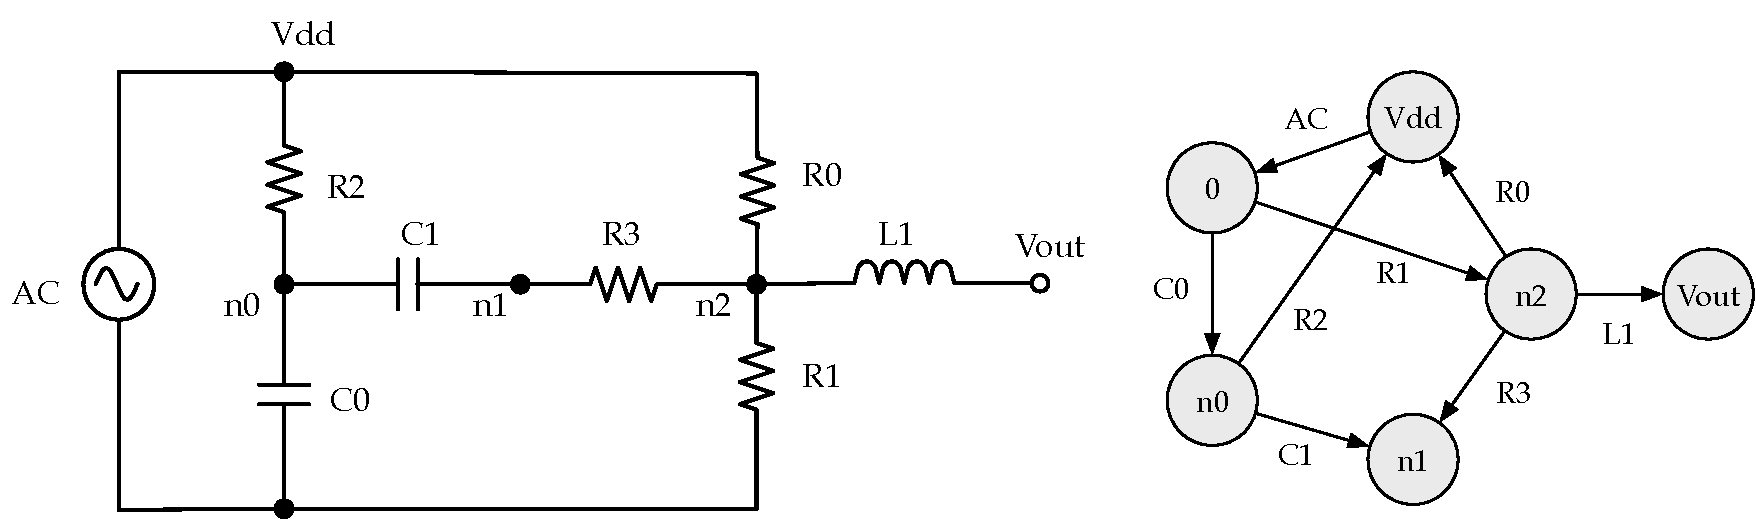
\includegraphics[width=0.56\textwidth]{figs/circuit.pdf}}
    \caption{Node and link graph models, an intuitive representation of relationships between entities.\label{fig:node_link_graphs}}
  \end{center}
\end{figure}

Associated with every $v_i \in V$ is the integer $i$. We call $i$ the \emph{index}
(or the \emph{vertex identifier}) of $v_i$. The index of a vertex is a unique
identifier for that vertex. The index of a vertex is not necessarily the same
as the position of the vertex in the vertex set $V$. For example, in the graph
$G = \{ \{ 0, 1, 2, 3 \}, \{ (0, 1), (1, 2), (2, 3) \} \}$, the vertex $v_0$ has index 0,
$v_1$ has index 1, $v_2$ has index 2, and $v_3$ has index 3. In the literature,
a vertex and its index are often used interchangeably.

A \emph{bipartite graph} is a graph $G$ with two disjoint sets of
vertices $U$ and $V$ such that every edge in $E$ connects a vertex
in $U$ to a vertex in $V$. A bipartite graph is useful for modeling
connections between two different types of objects. For example,
a bipartite graph can be used to model connections between
actors and movies that they have appeared in. To obtain
an actor-actor co-star graph from an actor-movie graph, we
perform a \emph{join} operation on the graph and its \emph{transpose}, which is
the graph connecting movies to actors, that is the graph with the same
vertices as the original graph but with edge directions reversed, i.e., a graph
connecting movies to actors (see Figure~\ref{fig:movie_actor}).

\begin{figure}[ht]
  \begin{center}
    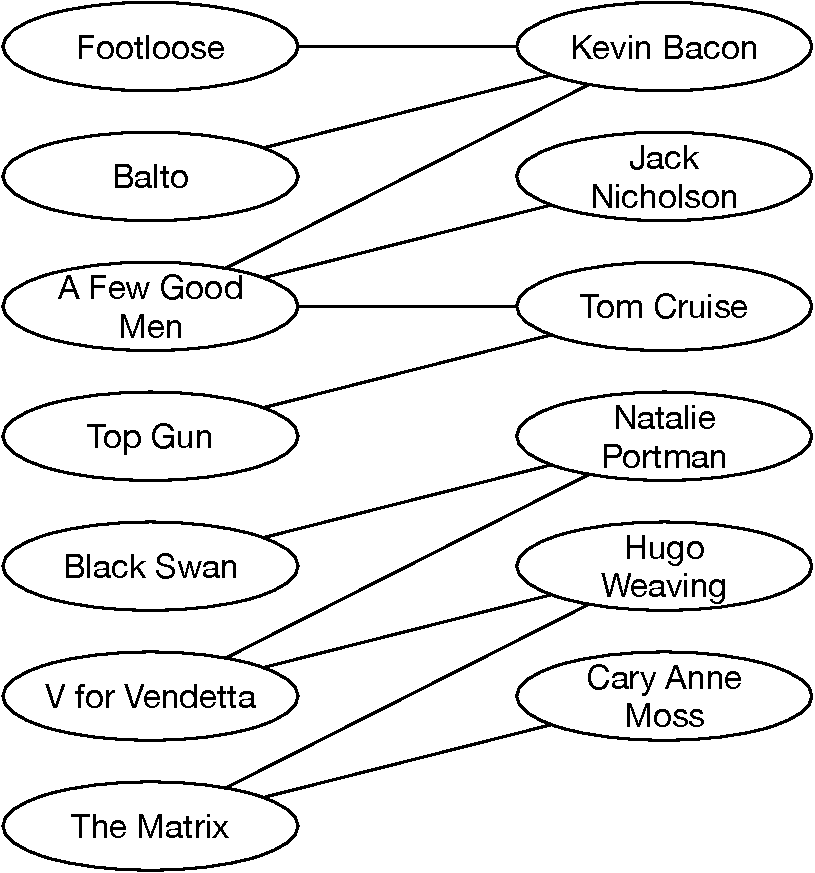
\includegraphics[width=0.25\textwidth]{movie_actor.pdf}\label{fig:movie_actor}
    \caption{A movie-actor graph. The links indicate that an actor has appeared in a movie.\label{fig:movie_actor}}
  \end{center}
\end{figure}

\subsection{Adjacency List}

An \emph{adjacency list} of $G$ is a data structure that represents a graph $G$ as an array
indexed by the vertex indices of the vertices of $G$.
The adjacency list of $G$ is denoted as $Adj(G)$.
For each vertex $v_i \in G$, the array entry $Adj(G)[i]$ is a list of
vertex indices of the vertices adjacent to $v_i$.
The adjacency list is the most common representation of a graph in the graph literature
and is used in the majority of graph algorithms as it has the important
property for traversal that (in the case of a unipartite graph)
an index $j$ stored neighbor list $Adj(G)[i]$ can
be used to index back into $Adj(G)$. In this formulation, the adjacency list
does not store vertices per se (rather, it stores vertex indices), it captures the
structure of the graph. This structure is the essence of the graph abstraction and
is the essential information needed for graph algorithms.
Even so, it is still possible to store vertex data in the adjacency list by storing
the vertex data in an auxiliary array indexed by vertex indices.

\subsection{Edge List}

An \emph{edge list} of $G$ is a data structure that contains the edges of $G$. More precisely, as
with the adjacency list structure, the edge list stores pairs of vertex indices. That is, for
every $(v_i, v_j) \in E$, the edge list contains the pair $(i, j)$. The edge list is
a less common representation of a graph than the adjacency list, but it is useful for
some graph algorithms. Moreover, it is a natural intermediate representation for
converting between data that has not yet been interpreted as a graph, e.g., a table,
and an adjacency list. Moreover, certain tasks, such as sorting or relabeling vertices, are
more natural to express in terms of the edge list.

\subsection{Adjacency Matrix}

\andrew{Is this useful? Should it be included in std::graph?
I personally don't think it is very useful, but the committee may disagree
since it is often used in the literature (typically introductory).}


\section{From Data to Graph}

\subsection{Columnar Data}

Figure~ref{fig:edge\_list\_from\_columnar\_data}
shows how one might create an unlabeled edge list from a table of data stored in a CSV file.
The values in each row are assumed to be separated by whitespace.
The elements of the first column are considered to be the source vertices and the elements of
the second column are the destination vertices. For edges with properties, the third column
contains the property values.

\begin{figure}[ht]
  \begin{center}
    \begin{subfigure}{0.48\textwidth}
      \begin{lstlisting}[language=C++]
    auto directed_edge_list<vertex_id_t, vertex_id_t>
      std::vector<std::tuple<vertex_id_t, vertex_id_t> edges;
    auto input = std::ifstream ("input.csv");
    vertex_id_t src, dst;
    while (input >> src >> dst) {
        edges.emplace_back (src, dst);
    }
      \end{lstlisting}
      \caption{Creating a directed edge list with no edge properties.
      The edge list container is a vector of tuples.
      \label{subfig:edge_list_no_properties}}
    \end{subfigure}
    \begin{subfigure}{0.48\textwidth}
      \begin{lstlisting}[language=C++]
    auto undirected_edge_list_graph<vertex_id_t, vertex_id_t, double>
      graph<std::vector<vertex_id_t>, std::vector<vertex_id_t>, std::vector<double>> edges;
    auto input = std::ifstream ("input.csv");
    vertex_id_t src, dst;
    double val;
    while (input >> src >> dst >> val) {
        edges.emplace_back (src, dst, val);
    }
      \end{lstlisting}
      \caption{Creating an undirected edge list with edge properties.
      The edge list container is comprised of three vectors, wrapped by
      the `lstinline{graph}' adapter.
      \label{subfig:edge_list_with_properties}}
    \end{subfigure}
    \caption{Creating an edge list from columnar data.\label{fig:edge_list_from_columnar_data}}
  \end{center}
\end{figure}

These examples are meant to be illustrative and not necessarily
comprehensive (nor efficient).
There are, of course, many ways to define containers that meet the
requirements of the edge list concept and many ways to
create an edge list from columnar data.

\subsection{Converting an Edge List to an Adjacency List}

\begin{figure}[ht]
  \begin{center}
    \begin{subfigure}{0.48\textwidth}
      \begin{lstlisting}[language=C++]
    auto edge_list<vertex_id_t, vertex_id_t> std::vector<std::tuple<vertex_id_t, vertex_id_t> edges;
    auto adjacency_list<vertex_id_t> std::vector<std::vector<vertex_d_t>> adj_list;
    for (auto [src, dst] : edges) {
      if (src >= adj_list.size()) {
        adj_list.resize(src + 1);
      }
      adj_list[src].push_back (dst);
    }
      \end{lstlisting}
      \caption{Creating an adjacency list from a directed edge list.
      The adjacency list container is a vector of vectors.
      \label{subfig:adj_list_from_directed_edge_list}}
    \end{subfigure}
    \begin{subfigure}{0.48\textwidth}
      \begin{lstlisting}[language=C++]
    auto edge_list_graph<vertex_id_t, vertex_id_t>
      graph<std::vector<std::tuple<vertex_id_t, vertex_id_t>> edges;
    auto adjaceny_list_graph<vertex_id_t, vertex_id_t, double>
      graph<std::vector<std::vector<vertex_d_t>, std::vector<double>> adj_list{edges.num_vertices()};
    for (auto [src, dst, val] : edges) {
      adj_list[src].push_back (dst, val);
      adj_list[dst].push_back (src, val);
    }
      \end{lstlisting}
      \caption{Creating an adjacency list from an undirected edge list with properties.
      Since the edges in the edge list are undirected, for a given edge $(u, v, w)$,
        $u$ is a neighbor of $v$ and $v$ is a neighbor of $u$. Thus, we insert both
        $(u, v, w)$ and $(v, u, w)$ into the adjacency list.
        The adjacency list container is comprised of three vectors, wrapped by
        the `lstinline{graph}' adapter.
        \label{subfig:adj_list_from_undirected_edge_list}}
    \end{subfigure}
    \caption{Creating an adjacency list from an edge list with properties.\label{fig:adj_list_from_edge_list}}
  \end{center}
\end{figure}

\andrew{We should have note that anything wrapped in a graph adapter has a `num\_vertices`
method (and other members).
We should also provide a constructor for the adapted adjacency list that takes and
edge list as argument.}


% The examples above basically cover what I intened here.  Though perhaps we should
% explain in some more detail about what the concepts do, what kinds of things meet
% concept requirements, what the graph adapter does, etc.
% \section{Implementations}
% But maybe we can just cover those things further down and forward reference to
% them from here.

% \subsection{Edge List: Array of Structs / Struct of Arrays}
% \andrew{Edges can be stored as tuples (or tuple like) basically in parallel arrays (like a ranges::zip).}
% \subsection{Vertices and Edges: Node Objects and Link Objects}
% \andrew{ala Stanford Graph Base (et al).}
% \subsection{Adjacency List: Container of Containers}
% \andrew{An adjacency list can be represented as a container of containers (e.g., std::vector<std::list>).  Talk about range of ranges when we talk about library interfaces, requirements, concepts.  Note here that the structure of an adjacency list does not capture directedness -- directedness is a run-time property.}


% These are definitely already covered in the examples above.
% \subsection{From Edge List to Adjacency List}
% \andrew{Scan edge list and insert edgest into adjacency list.  Adjacency list must support insertion.}
% \subsection{Edge List and Adjacency List: Compressed Edge List}
% \andrew{Using a sort and group-by (or a sort, a run-length encoding, and a scan), we can compactify the edge-list reprentation and at the same time obtain an adjacency-list representation -- one that is memory and compute efficient.  Best of both worlds.  Has same basic structural principles as CSR / CSC matrices in linear algebra -- but much more general.}


\section{BiPartite Graphs}

So far, we have been considering graphs where the vertices, and both elements of an
edge, are members of a single set $|V|$. A graph with a single vertex set is called a
\emph{unipartite} graph. If the vertices in a graph can be partitioned into two
disjoint sets such that all of the edges in the graph only connect vertices from one
set of the vertices of the other set, the graph is called a \emph{bipartite} graph.

Even if a graph is designated to be unipartite, it may be the case that its vertices
can be partitioned into two disjont sets. In such a case, the graph is bipartite,
but as a run-time property, not a compile-time property.
That is, determining whether a given graph is bipartite requires a run-time analysis
of the graph, with an appropriate algorithm.

However, there are numerous cases of interest where the vertices of a graph fall
naturally into two disjoint sets. For example, in the
in a social network, the vertices
represent people and the edges represent friendships. In such a case, it is natural
Of particular interest for realizing a bipartite graph is when the graph is
structurally bipartite, that is, when we are explicitly given two different
sets of vertices and the corresponding set of edges that connect vertices of the two sets.
This common---and important---use case arises when modeling relationships
between different types of entities. For example, we might use a structurally
bipartite graph in which one vertex set represents customers and another vertex
set represents products. An edge between a customer and a product would be used
to indicate that a customer has purchased a particular product.
Another such example is from the Kevin Bacon game above, where
one set represents actors and the other set represents movies; edges represent whether
and actor appeared in a movie. Thus edges only connect vertices from the set of actors
to the set of movies.

We can refer to graphs of this form as \emph{structurally bipartite} graphs and
denote them as $G = (U, V, E)$, where the vertex sets $U$ and $V$ are disjoint.

\subsection{BiPartite Graph Models}

\subsection{BiPartite Graph Implementations}


\section{Relationship between Graphs and Sparse Matrices}


\section{Naming Conventions}


Table~\ref{tab:name_conv} shows the naming conventions used throughout this document.

\begin{table}[h!]
  \begin{center}
  {\begin{tabular}{l l l p{7cm}}
     \hline
     \textbf{Template}  &                                   & \textbf{Variable}    &                                                                                                                                                                                                  \\
     \textbf{Parameter} & \textbf{Type Alias}               & \textbf{Names}       & \textbf{Description}                                                                                                                                                                             \\
     \hline
     \tcode{G}          &                                   &                      & Graph                                                                                                                                                                                            \\
     & \tcode{graph_reference_t<G>}      & \tcode{g}            & Graph reference                                                                                                                                                                                  \\
     \tcode{GV}         &                                   & \tcode{val}          & Graph Value, value or reference                                                                                                                                                                  \\
     \hline
     \tcode{V}          & \tcode{vertex_t<G>}               &                      & Vertex                                                                                                                                                                                           \\
     & \tcode{vertex_reference_t<G>}     & \tcode{u,v,x,y}      & Vertex reference. \tcode{u} is the source (or only) vertex. \tcode{v} is the target vertex.                                                                                                      \\
     \tcode{VId}        & \tcode{vertex_id_t<G>}            & \tcode{uid,vid,seed} & Vertex id. \tcode{uid} is the source (or only) vertex id. \tcode{vid} is the target vertex id.                                                                                                   \\
     \tcode{VV}         & \tcode{vertex_value_t<G>}         & \tcode{val}          & Vertex Value, value or reference. This can be either the user-defined value on a vertex, or a value returned by a function object (e.g. \tcode{VVF}) that is related to the vertex.              \\
     \tcode{VR}         & \tcode{vertex_range_t<G>}         & \tcode{ur,vr}        & Vertex Range                                                                                                                                                                                     \\
     \tcode{VI}         & \tcode{vertex_iterator_t<G>}      & \tcode{ui,vi}        & Vertex Iterator. \tcode{ui} is the source (or only) vertex.                                                                                                                                      \\
     &                                   & \tcode{first,last}   & \tcode{vi} is the target vertex.                                                                                                                                                                 \\
     \tcode{VVF}        &                                   & \tcode{vvf}          & Vertex Value Function: vvf(u) $\rightarrow$ value                                                                                                                                                \\
     \hline
     \tcode{E}          & \tcode{edge_t<G>}                 &                      & Edge                                                                                                                                                                                             \\
     & \tcode{edge_reference_t<G>}       & \tcode{uv,vw}        & Edge reference. \tcode{uv} is an edge from vertices \tcode{u} to \tcode{v}. \tcode{vw} is an edge from vertices \tcode{v} to \tcode{w}.                                                          \\
     \tcode{EV}         & \tcode{edge_value_t<G>}           & \tcode{val}          & Edge Value, value or reference. This can be either the user-defined value on an edge, or a value returned by a function object (e.g. \tcode{EVF}) that is related to the edge.                   \\
     \tcode{ER}         & \tcode{vertex_edge_range_t<G>}    &                      & Edge Range for edges of a vertex                                                                                                                                                                 \\
     \tcode{EI}         & \tcode{vertex_edge_iterator_t<G>} & \tcode{uvi,vwi}      & Edge Iterator for an edge of a vertex. \tcode{uvi} is an iterator for an edge from vertices \tcode{u} to \tcode{v}. \tcode{vwi} is an iterator for an edge from vertices \tcode{v} to \tcode{w}. \\
     \tcode{EVF}        &                                   & \tcode{evf}          & Edge Value Function: evf(uv) $\rightarrow$ value                                                                                                                                                 \\
     \hline
  \end{tabular}}
    \caption{Naming Conventions for Types and Variables}
    \label{tab:name_conv}
  \end{center}
\end{table}

